\documentclass{article}
\usepackage{graphicx}
\usepackage{amsmath}
% Note: composable package will be auto-injected by cstex

\title{CSF Declarative Annotation Demo}
\author{CSF Team}
\date{\today}

\begin{document}

\maketitle

\section{Introduction}

This document demonstrates the new CSF Declarative Annotation system, which provides 
explicit control over computational metadata while maintaining plain LaTeX compatibility.

\section{Statistical Results with Declarative Annotations}

Our analysis revealed a strong correlation between temperature and pressure
(r = \csfvaluelink{main_correlation}{float,round2}).

This correlation is statistically significant (p < \csfvaluelink{significance_test}{scientific,round3}).

The mean temperature was \csfvaluelink{sample_mean}{float,round1}°C across all measurements.

Our predictive model achieved an accuracy of \csfvaluelink{model_accuracy}{percent,round1} on the test dataset.

\section{Figures with Declarative Metadata}

\begin{figure}[h]
\centering
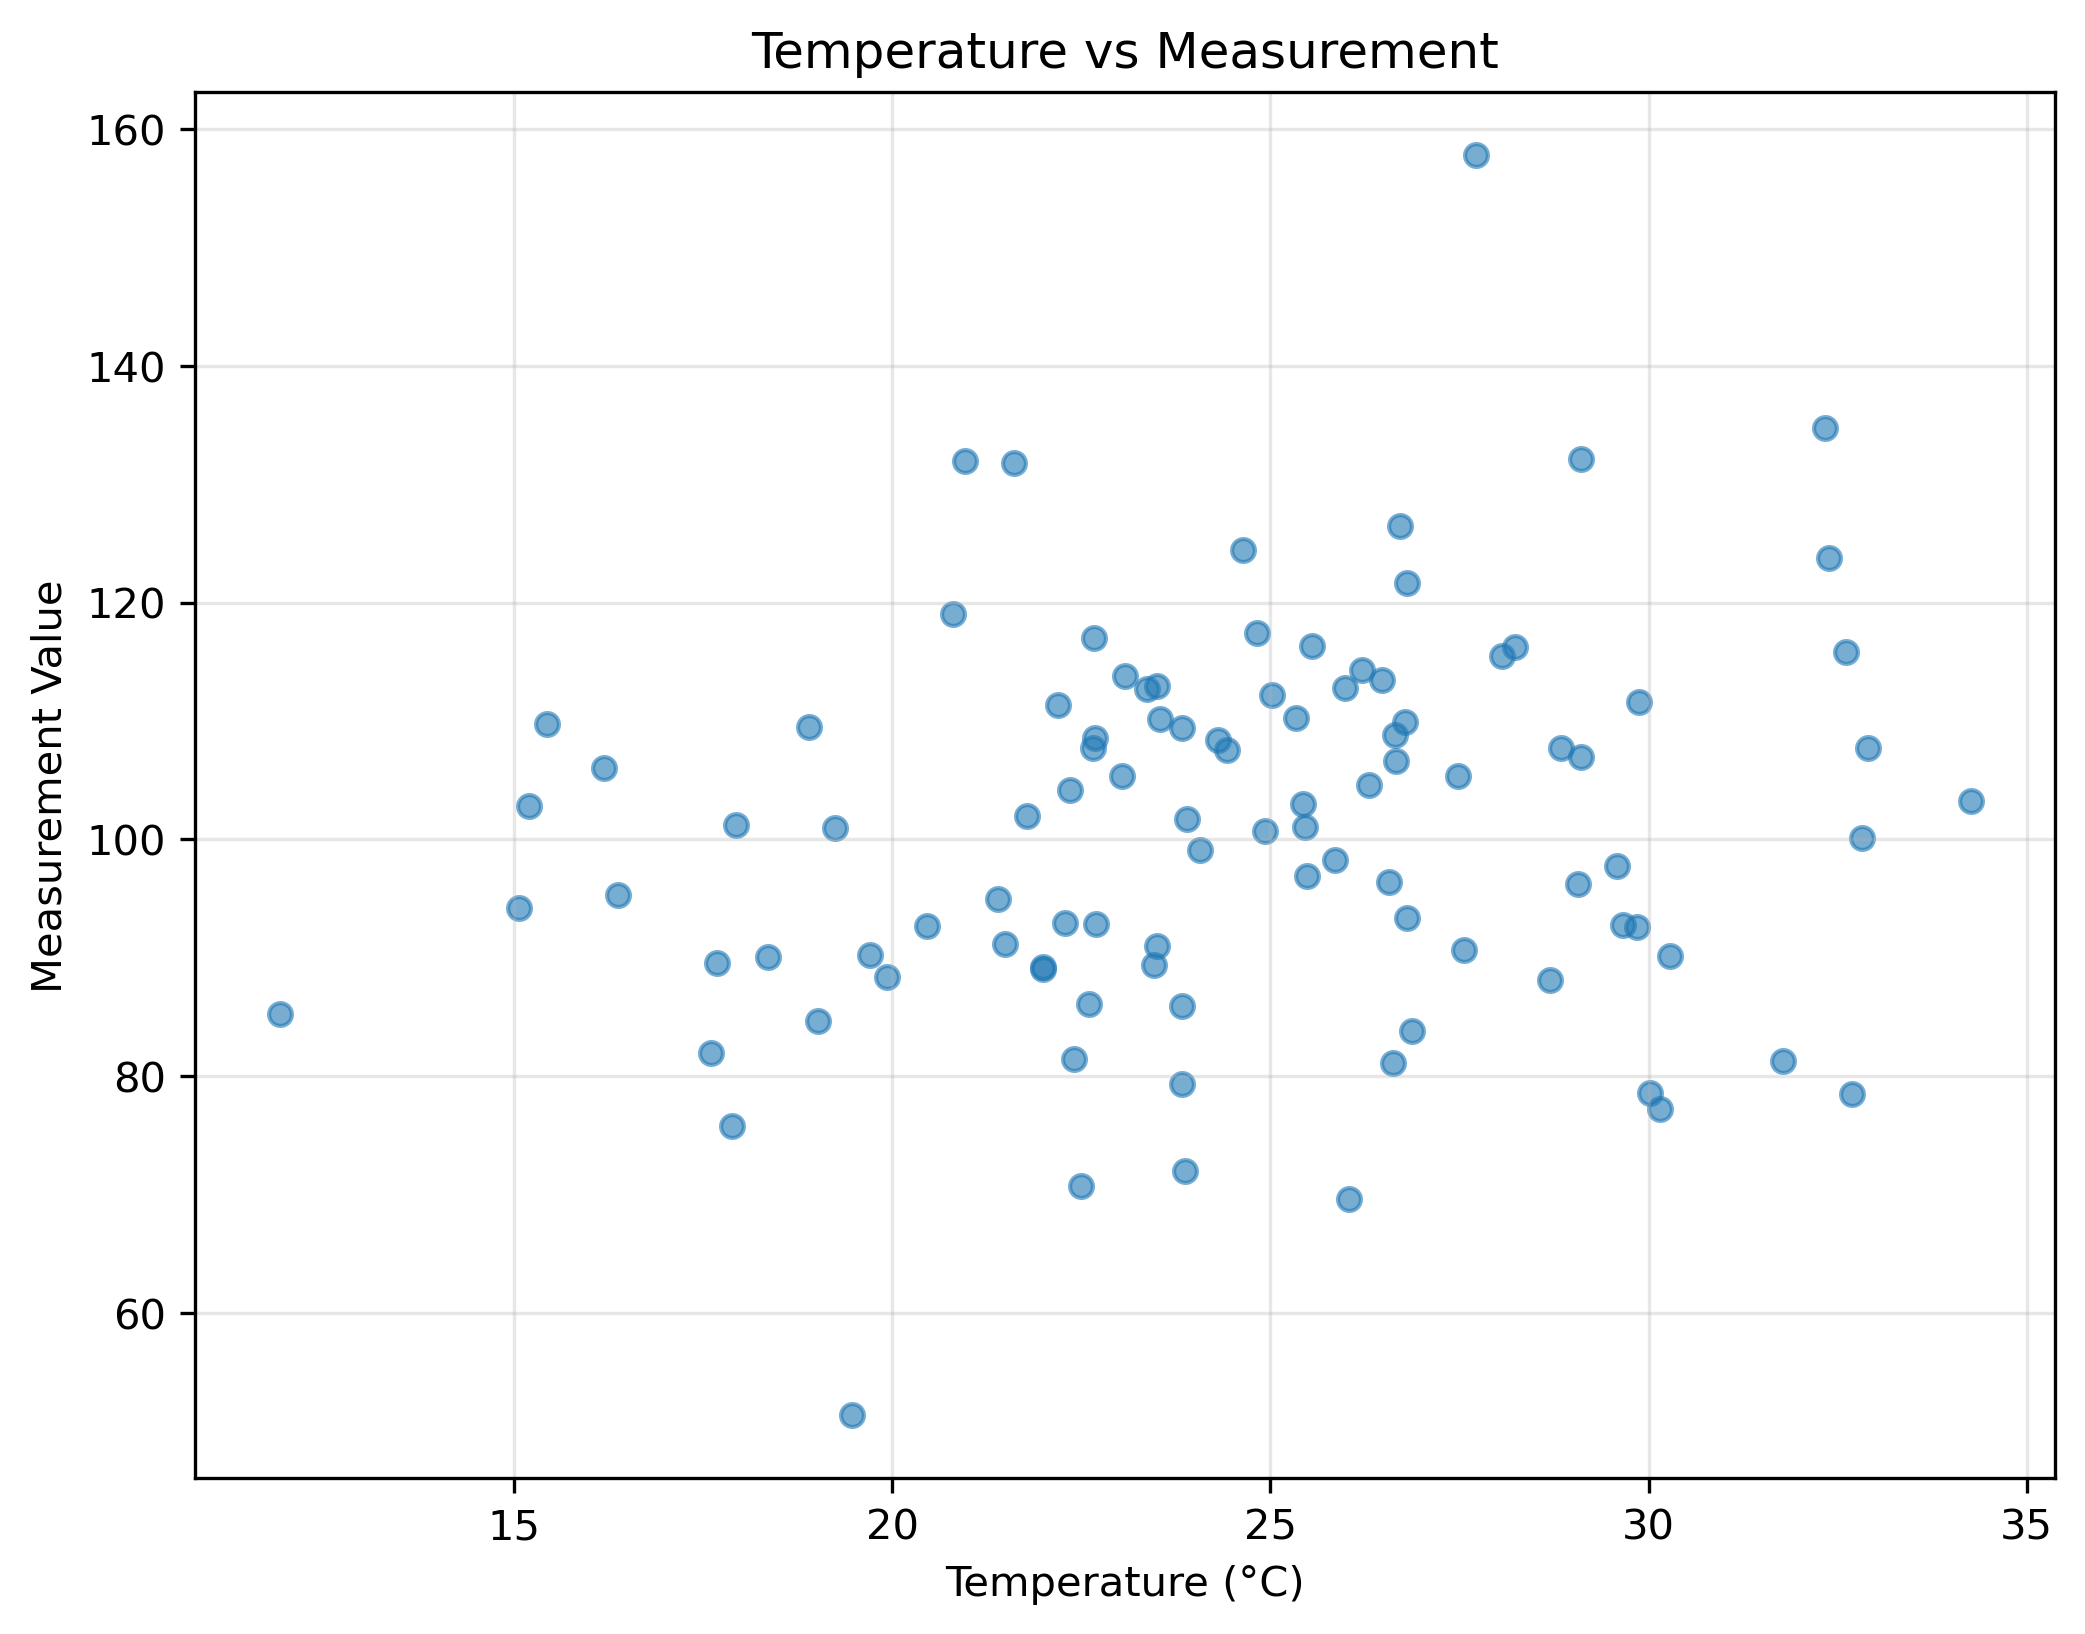
\includegraphics[width=0.8\textwidth]{figures/temperature_measurement.png}
\csflink{figures/temperature_measurement.png}
\caption{Temperature vs Measurement Analysis with explicit CSF metadata}
\label{fig:temp_declarative}
\end{figure}

The figure above (\ref{fig:temp_declarative}) uses declarative CSF annotations to specify 
exact provenance metadata, ensuring precise computational traceability.

\section{Data Tables with Declarative Linking}

\begin{table}[h]
\centering
\begin{tabular}{|l|r|r|}
\hline
Statistic & Value & Unit \\
\hline
Mean Temperature & 23.7 & °C \\
Std Deviation & 4.2 & °C \\
Sample Size & 1000 & measurements \\
\hline
\end{tabular}
\csflink{outputs/summary_stats.csv}
\caption{Summary statistics with declarative CSF table linking}
\label{tab:summary_declarative}
\end{table}

Table \ref{tab:summary_declarative} demonstrates how the \texttt{\\csftablelink} command 
provides provenance links to the computational source of tabular data.

\section{Mixed Automatic and Declarative Approach}

This section shows how automatic discovery and declarative annotations work together:

% Automatic discovery (no annotation needed)
\begin{figure}[h]
\centering
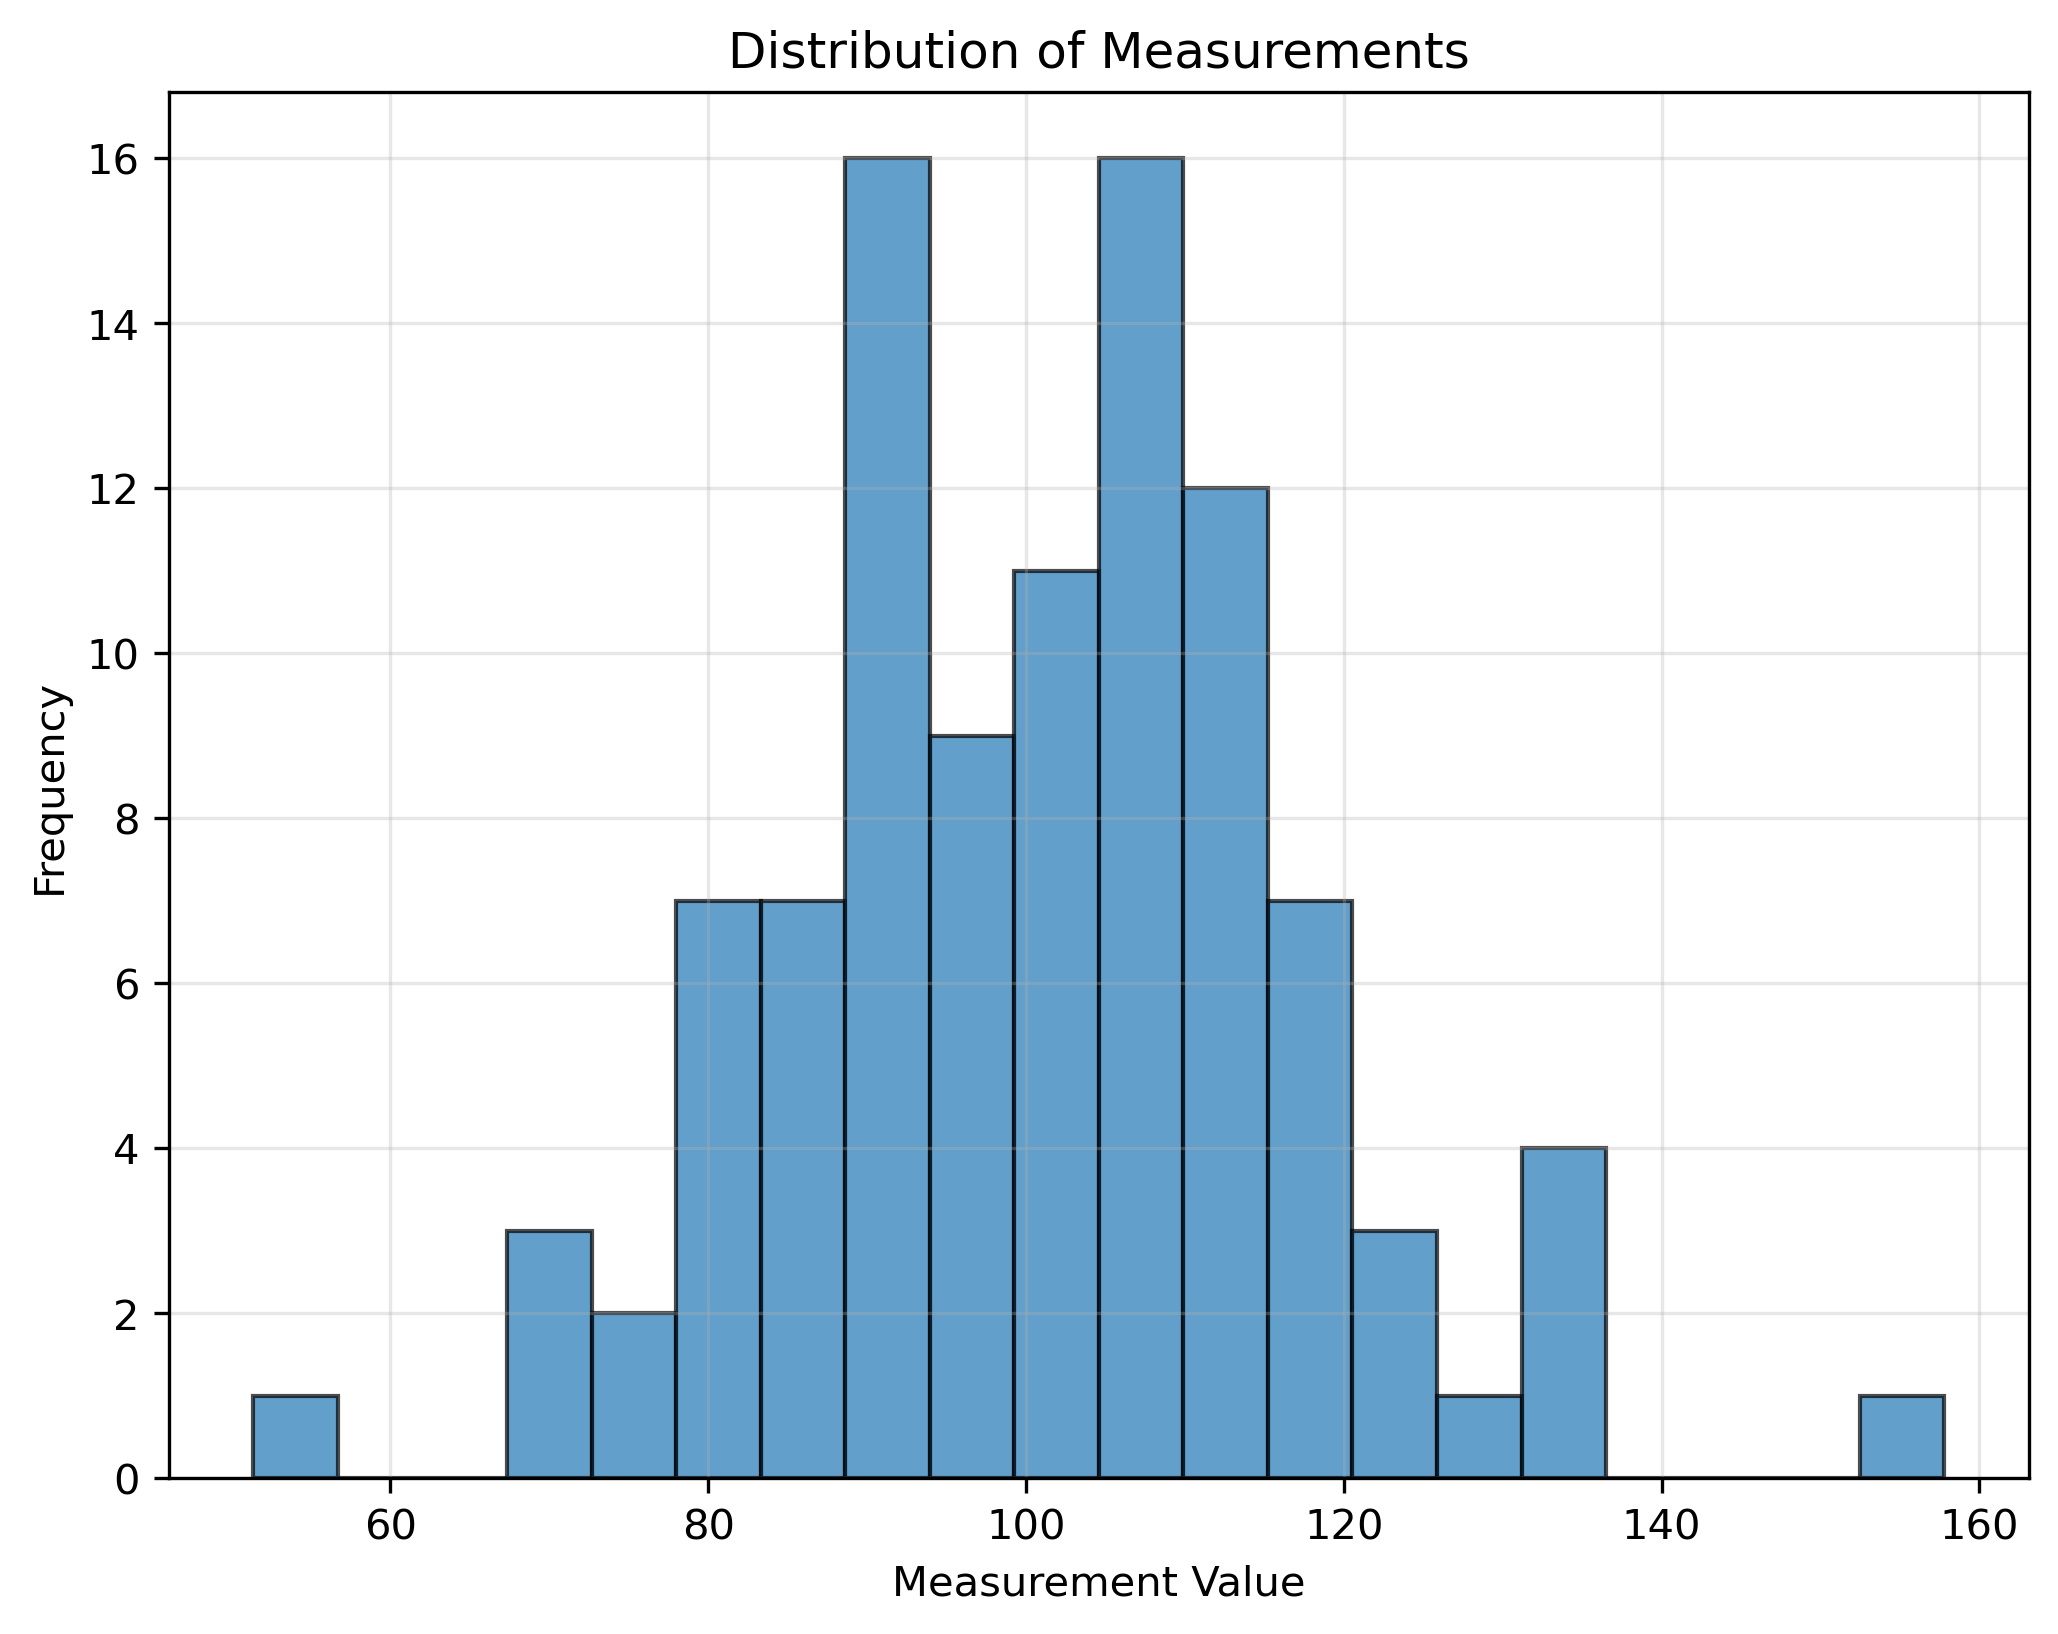
\includegraphics[width=0.7\textwidth]{figures/measurement_distribution.png}
\csflink{figures/measurement_distribution.png}
\caption{Distribution plot discovered automatically by CSF}
\label{fig:auto}
\end{figure}

% The custom_analysis.png figure does not exist, so it has been removed for this test.

\section{Compatibility Notes}

\subsection{Plain LaTeX Compilation}

When compiled with standard LaTeX (without CSTeX):
\begin{itemize}
    \item CSF comment annotations are ignored (invisible)
    \item \texttt{\\csfstatlink\{name\}\{format\}} shows the format specifier
    \item \texttt{\\csftablelink} commands are invisible
    \item Document compiles normally with placeholders
\end{itemize}

\subsection{CSTeX Enhanced Compilation}

When compiled with CSTeX:
\begin{itemize}
    \item Values are extracted from pipeline execution
    \item Statistical outputs show computed values with provenance links
    \item All artifacts link to dashboard for verification
    \item Full computational transparency is enabled
\end{itemize}

\section{Conclusion}

The CSF Declarative Annotation system provides the best of both worlds:
\begin{enumerate}
    \item \textbf{Zero-configuration} for simple cases (automatic discovery)
    \item \textbf{Explicit control} for complex scenarios (declarative annotations)
    \item \textbf{Plain LaTeX compatibility} through fallback commands
    \item \textbf{Runtime value injection} for fresh computational results
\end{enumerate}

This approach enables computational transparency that scales from simple documents 
to complex multi-step analytical workflows.

\end{document}